\chapter{Νευρωνικά Δίκτυα για Εντοπισμό Αντικειμένων}%
\label{chapter:neuralNets}
\section{Εισαγωγή}
Τα τελευταία χρόνια έχει προταθεί ένας μεγάλος αριθμός νευρωνικών δικτύων για τον εντοπισμό αντικειμένων από εικόνες. Η εισαγωγή της έννοιας του CNN, όπου πρόκειται για νευρωνικό δίκτυο το οποίο έχει επίπεδα που εκτελούν συνελίξεις για την αναγνώριση χειρόγραφων αριθμών είχε ήδη προταθεί το 1998 \cite{36} και το 2006 \cite{35}. Ωστόσο, λόγω υψηλής απαίτησης σε υπολογιστική ισχύ δεν προτεινόταν η χρήση τους στην επίλυση προβλημάτων αναγνώρισης αντικειμένων ή εντοπισμό. Η αλλαγή της πορείας έγινε το 2012, όταν προτάθηκε το AlexNet \cite{20} το οποίο είναι ένα νευρωνικό δίκτυο πολλών επιπέδων (deep) το οποίο έχει επίπεδα συνελίσουν την είσοδό τους με τα βάρη τους (convolutional). Με αυτό παρουσιάζονται και οι δύο συγκυρίες που έδωσαν ώθηση στη βαθιά μηχανική μάθηση - τα σύνολα δεδομένων (π.χ. ImageNet) και η υπολογιστική ισχύς των GPU (η εκπαίδευση είναι πλέον εφικτή σε σχετικά μικρό χρόνο). Από τότε και έπειτα άρχισε η χρήση και η δημιουργία καινούριων CNN για προβλήματα που εμπεριέχουν την αναγνώριση και τον εντοπισμό αντικειμένων. Τα δίκτυα που προτάθηκαν το δεύτερο μισό του 2017 και μόνο για την αναγνώριση/εντοπισμό αντικειμένων ξεπερνούν τα δέκα. Επιπλέον η απαίτηση χρήση τους σε πραγματικού χρόνου εφαρμογές και σε ενσωματωμένα συστήματα έδωσε μια άλλη οπτική ανάπτυξής τους. Σε αυτό το κεφάλαιο αναλύονται τα σημαντικότερα δίκτυα που αποτελούν ορόσημα για την χρήση των νευρωνικών σε ενσωματωμένες συσκευές.

% Template of a new CNN-net
% Title: A new net 
% Contents:
% 1. When was proposed
% 2. What makes it special for detection
% 3. Architecture descritpion
% 4. Training & Retraining
% 5. Accuracy
% 6. Speed
% 7. Memory
% 8. Energy consumption
% 9.”Is it good for embedded systems?”

\section{SqueezeDet-Net \cite{1} \cite{2}}
Τα δίκτυα αυτά προτάθηκαν από ερευνητές του πανεπιστημίου του Berkeley και της εταιρίας Deepscale ως μια λύση για το πρόβλημα του μεγάλου αριθμού παραμέτρων ενός νευρωνικού δικτύου για εντοπισμό αντικειμένων. Το SqueezeΝet ουσιαστικά εμπεριέχεται στο SqueezeDet ως ένα από τα επίπεδά του. Και τα δύο προτάθηκαν για επίλυση προβλημάτων που αφορούν την αυτοκινητοβιομηχανία. Η μείωση του αριθμού των παραμέτρων κάνει εφικτή την αναγνώριση αντικειμένων σε πραγματικό χρόνο και επιτυγχάνει μεγαλύτερη ενεργειακή αποδοτικότητα. Σε σύγκριση με το AlexNet\cite{20}, επιτυγχάνει την ίδια ακρίβεια με 50x μικρότερο μέγεθος παραμέτρων. Η είσοδος που δέχεται είναι το ήδη επεξεργασμένο αποτέλεσμα του SqueezeNet.

\begin{figure}[H]
\centering
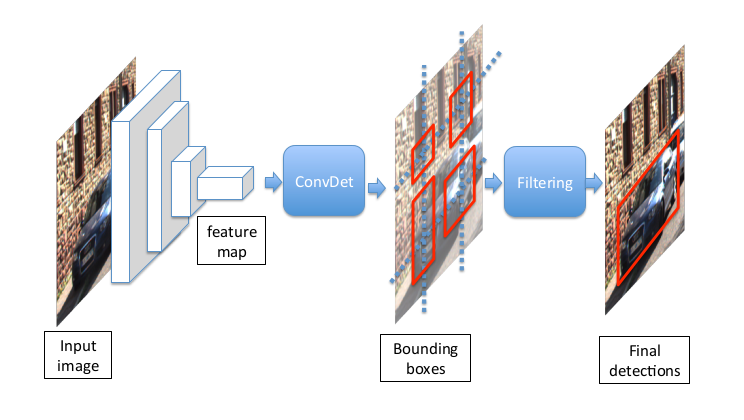
\includegraphics[width = \textwidth]{figures/SqueezeNetDet/SqueezeDet_architecture.png}
\caption[Αρχιτεκτονική SqueezeDet]{Η σειρά επεξεργασίας του SqueezeDet για εντοπισμό αντικειμένων. Ένα CNN π.χ. SqueezeNet εξάγει χαρακτηριστικά από την εικόνα εισόδου και τα δίνει ως είσοδο στο επίπεδο ConvDet. Με τη σειρά του, το επίπεδο ConvDet υπολογίζει τα ορθογώνια περιβλήματα γύρω από τα ομοιόμορφα κατανεμημένα $ W\times H$ κέντρα των πιθανών αντικειμένων. Κάθε ορθογώνιο περίβλημα σχετίζεται με $1$ σκορ εμπιστοσύνης και $C$ υπό συνθήκη πιθανότητες. Κατά το επίπεδο \textit{Filtering} κρατούνται τα $N$ περιβλήματα με τα κυρίαρχα σκορ εμπιστοσύνης και χρησιμοποιούνται αλγόριθμοι \textit{NMS} για τη λήψη των τελικά εντοπισμένων αντικειμένων.}
\label{fig:SqueezeDet_architecture}
\end{figure}


Η αρχιτεκτονική του SqueezeDet, του επιτρέπει να προτείνει την ορθογώνια περιοχή μέσα στην οποία εντοπίζει ένα αντικείμενο σε μία εικόνα αλλά και να το κατηγοριοποιεί ταυτόχρονα. Ουσιαστικά αποτελείται από ένα επίπεδο συνελίξεων το οποίο προτείνει τις περιοχές ύπαρξης αντικειμένων και ένα NMS (Non-Maximum Suppression) φίλτρο για υπολογισμό της πιθανότητας ύπαρξης κάποιου αντικειμένου στις προτεινόμενες περιοχές. Το φίλτρο εφαρμόζεται σε όλη την έξοδο του ConvNet και η πιθανότητα υπολογίζεται από τον τύπο:
$$ max \{ Pr\left(class_C| Object\right)\} * Pr(Object) * IOU^{pred}_{truth} $$

To SqueezeNet με τη σειρά του αποτελεί ιδανική υλοποίηση του επιπέδου συνελίξεων του SqueezeDet γιατί στοχεύει στον μικρό αριθμό παραμέτρων. Επίσης, κατά τη σχεδίασή του δόθηκε περισσότερη έμφαση στον διανυσματικό χώρο των βαρών με δεδομένη ακρίβεια και όχι το ανάποδο. Αυτό ήταν που οδήγησε στις παρακάτω τρεις στρατηγικές για τη μείωση του αριθμού των παραμέτρων:

\begin{enumerate}
    \item Αντικατάσταση των $3\times3$ φίλτρων με $1\times1$.
    \item Μείωση του αριθμού καναλιών στα $3\times3$ φίλτρα, με χρήση επιπλέον επιπέδων (\textit{squeeze layers}).
    \item H υποδειγματοληψία γίνεται στα τελευταία layers του δικτύου.
\end{enumerate}

Με εφαρμογή αυτών των τριών στρατηγικών και με υλοποίηση της λογικής "Network in Network"\cite{75} των ResNet \cite{21} και GoogleNet \cite{24} το νευρωνικό αποτελείται από μικρότερες οντότητες, οι οποίες ονομάζονται \textit{fire modules}. Κάθε τέτοια οντότητα όπως φαίνεται στο Σχήμα \ref{fig:SqueezeNet_microarchitecture} ορίζεται από τις παραμέτρους:
\begin{itemize}
  \setlength\itemsep{0em}
    \item {$ s_{1 \times 1} $ ο αριθμός φίλτρων στο \textit{squeeze layer}}
    \item {$ e_{1 \times 1} $ o αριθμός $ 1\times1 $ φίλτρων στο \textit{expand layer}}
    \item {$ e_{3 \times 3} $  o αριθμός $ 3\times3 $ φίλτρων στο \textit{expand layer}}
\end{itemize}

Προκειμένου να επιτευχθεί η στρατηγική 2 απαιτείται $s_{1\times1} < (e_{1\times1} + e_{3\times3})$. Έπειτα ολόκληρη η αρχιτεκτονική αποτυπώνεται καλύτερα στο Σχήμα \ref{fig:SqueezeNet_microarchitecture}. Επιπλέον %χρησιμοποιείται η τεχνική \textit{dropout} \cite{3} με ποσοστό 50\% και 
στην είσοδο των $3\times3$ φίλτρων γίνεται \textit{zero-padding} κατά $1$ εικονοστοιχείων στο σύνορο.

Η εκπαίδευση του δικτύου γίνεται με \textit{Stochastic Gradient Descent} χρησιμοποιώντας την ίδια συνάρτηση κόστους που χρησιμοποιεί το δίκτυο YOLO\cite{6}. Κατά την εκκίνηση το learning rate είναι 0.04, το οποίο μειώνεται κατά την πάροδο των εποχών. Στο τέλος της εκπαίδευσης μπορεί να εφαρμοστεί και η τεχνική Deep Compression στο SqueezeNet με την οποία χρησιμοποιώντας μόνο 0.66 ΜΒ επιτυγχάνεται ακρίβεια 80.3\% στα 6 bit στο σύνολο δεδομένων του ImageNet. Η συνάρτηση κόστους εκπαιδεύει και τα 2 επίπεδα της αρχιτεκτονικής:

% \begin{figure}[H]
% \centering
% 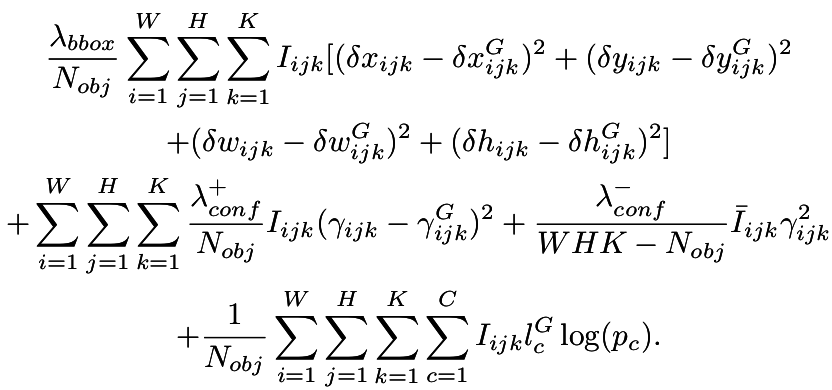
\includegraphics[width = \textwidth]{figures/SqueezeNetDet/SqueezeDet_lossFunction.png}
% \end{figure}

$$
\frac{\lambda_{bbox}}{N_{obj}} \sum_{i=1}^{W} \sum_{j=1}^{H} \sum_{k=1}^{K} I_{ijk} \left[(\delta\chi_{ijk} - \delta\chi_{ijk}^{G})^2 + ({\delta y}_{ijk} - {\delta y}_{ijk}^{G})^2 \right.
$$

$$
\left. + ({\delta w}_{ijk} - {\delta w}_{ijk}^{G})^2 + ({\delta h}_{ijk} - {\delta h}_{ijk}^{G})^2\right]
$$

$$
+ \sum_{i=1}^{W} \sum_{j=1}^{H} \sum_{k=1}^{K} \frac{\lambda_{conf}^{+}}{N_{obj}} I_{ijk} (\gamma_{ijk} - \gamma_{ijk}^G)^2 + \frac{\lambda_{conf}^{-}}{W H K - N_{obj}} \bar{I}_{ijk}\gamma_{ijk}^{2}
$$

$$
 + \frac{1}{N_{obj}} \sum_{i=1}^{W} \sum_{j=1}^{H} \sum_{k=1}^{K} \sum_{c=1}^{C} I_{ijk}l_{c}^{G}\log(p_c)
$$

Το πρώτο κομμάτι είναι για την εύρεση του περιβλήματος των αντικειμένων. Το σημείο $({\delta x}_{ijk}, {\delta y}_{ijk}, {\delta w}_{ijk}, {\delta h}_{ijk})$ αφορά τις σχετικές συντεταγμένες του πιθανού περιβλήματος ως προς το σημείο $(i,j)$. Το δεύτερο κομμάτι (η γραμμή με το δεύτερο τριπλό άθροισμα) αφορά την παλινδρόμηση για το σκορ εμπιστοσύνης. Έπειτα, το τρίτο κομμάτι αφορά την cross-entropy για κατηγοριοποίηση των αντικειμένων σε κλάσεις.
Η ακρίβεια του αλγορίθμου υπολογίστηκε πάνω στο σύνολο δεδομένων του KITTI και δίνεται με το κριτήριο (mAP) για τους πεζούς, τα αυτοκίνητα και τους ποδηλάτες.

\begin{tabular}{|*{10}{c|}} 
\hline
Μέθοδος & \multicolumn{3}{c|}{Car} & \multicolumn{3}{c|}{Cyclist} & \multicolumn{3}{c|}{Pedestrian}\\
\hline
SqueezeDet & 90.2 & 84.7 & 73.9 & 82.9 & 75.4 & 72.1 & 77.1 & 68.3 & 65.8 \\
SqueezeDet+ & 90.4 & 87.1 & 78.9 & 87.6 & 80.3 & 78.1 & 81.4 & 71.3 & 68.5 \\
\hline
\end{tabular}

\begin{tabular}{|*{3}{c|}}
\hline
Μέθοδος & Model size (MB) & mAP \\
\hline
SqueezeDet & 7.9 & 76.7\\
SqueezeDet+ & 26.8 & 80.4\\
\hline
\end{tabular}

Η απαίτηση μνήμης παρά τον παραπάνω πίνακα μπορεί να μειωθεί περαιτέρω. Με τη χρήση τεχνικών συμπίεσης και επηρεάζοντας τις υπερπαραμέτρους επιτυγχάνεται παραπάνω από $95\times$ συμπίεση κρατώντας την ίδια ευαισθησία. Ταυτόχρονα κερδίζει σε ταχύτητα και κατανάλωση ενέργειας. Μπορεί να φτάσει έως και τα 57.2 FPS στο KITTI, ενώ η ενισχυμένη εκδοσή του (SqueezeDet+) τα 32.1 FPS. Ο μειωμένος αριθμός παραμέτρων οδηγεί σε λιγότερη προσπέλαση μνήμης και οπότε λιγότερη χρήση της DRAM. Αυτή με τη σειρά της οδηγεί σε χαμηλότερη κατανάλωση ενέργειας είναι από 1.4 έως 4.0J/frame στο ΚΙΤΤΙ ανάλογα την έκδοση του SqueezeDet.

Ο χρόνος εκτέλεσης μειώνεται και αυτός με τη μείωση του αριθμού των παραμέτρων του δικτύου. Αν και στο ίδιο το έγγραφο που πρωτοπαρουσιάζεται το δίκτυο δε γίνεται λόγος για αυτό, η ενέργεια που καταγράφεται σε ενσωματωμένες συσκευές στο \cite{5}  είναι 26.37 J/frame στην πλατφόρμα του Nexus 5 για την εκτέλεση του SqueezeNet μόνο. Μάλιστα η παράλληλη υλοποίησή του οδηγεί σε ακόμα μικρότερη κατανάλωση ενέργειας. Για την ίδια πλατφόρμα έχει 249.47X λιγότερες ενεργειακές απαιτήσεις. Τέλος, η απαίτηση μνήμης, η κατανάλωση ενέργειας και η χρονική απόκριση του νευρωνικού, το χρήζουν κατάλληλο για ενσωματωμένα συστήματα.

\begin{figure}[H]
\centering
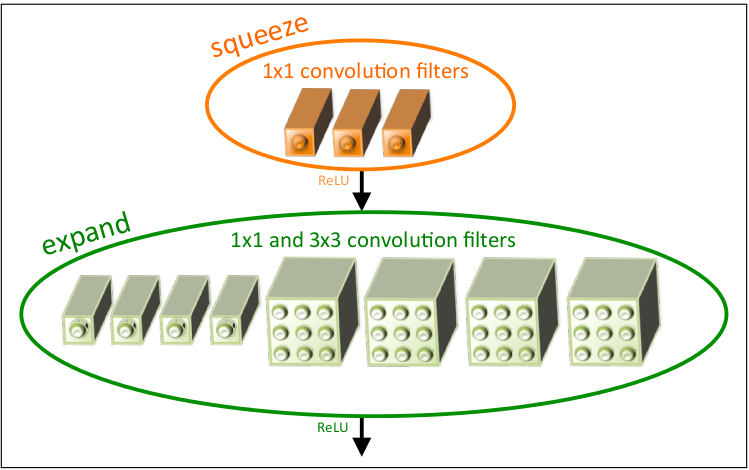
\includegraphics[width = \textwidth]{figures/SqueezeNetDet/SqueezeNet_microarchitecture.png}
\caption[Αρχιτεκτονική Fire module]{Μικροσκελής όψη της αρχιτεκτονικής SqueezeNet \cite{1}. Στην εικόνα φαίνεται το \textit{Fire module}, το οποίο είναι η βασική οντότητα όλου του SqueezeNet. Σε αυτό το παράδειγμα, $ s_{1x1} = 3, e_{1x1} = 4, e_{3x3} = 4$.}
\label{fig:SqueezeNet_microarchitecture}
\end{figure}

\begin{figure}[H]
\centering
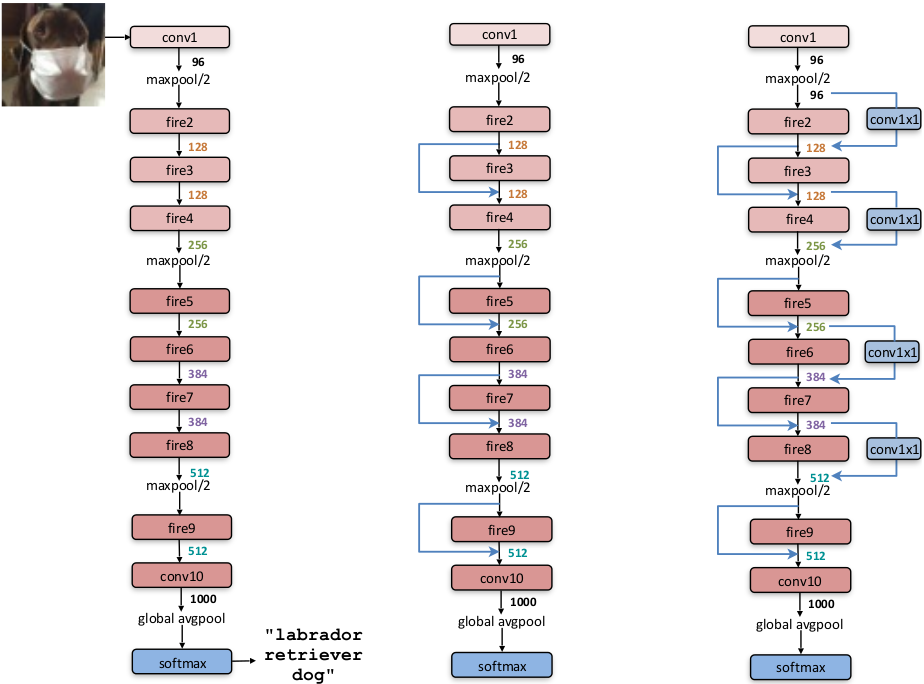
\includegraphics[width = \textwidth]{figures/SqueezeNetDet/SqueezeNet_macroarchitecture.png}
\caption[Αρχιτεκτονική SqueezeNet]{Μακροσκελής όψη της αρχιτεκτονικής SqueezeNet \cite{2}. Τα δίκτυα που παρουσιάζονται είναι τα: απλό SqueezeNet (αριστερά), SqueezeNet με απλό \text{bypass} (μέση), SqueezeNet με σύνθετο \text{bypass} (δεξιά). Η σύνδεση προηγουμένων επιπέδων με το επόμενο και όχι μόνο του αμέσως προηγούμενου ωφελεί την ακρίβεια του δικτύου.}
\label{fig:SqueezeNet_macroarchitecture}
\end{figure}



\section{YOLO\cite{6}}

Το δίκτυο αυτό προτάθηκε ως μια λύση για το πρόβλημα της πραγματικού χρόνου αναγνώρισης αντικειμένων διατηρώντας όσο το δυνατόν μεγαλύτερη μέση ακρίβεια. Χαρακτηρίζεται από το όνομά του \textit{You Only Look Once} που υποδηλώνει πως τόσο κατά τον εντοπισμό/αναγνώρισή όσο και κατά την εκπαίδευση, το δίκτυο λαμβάνει την εικόνα εισόδου μία φορά και δεν την επεξεργάζεται ξανά μετά την είσοδο κατά την εκτέλεση του. Οπότε, λαμβάνεται υπόψιν και η κατά το δυνατόν γρηγορότερη εκπαίδευση του. Οι ικανότητες του πέρα από την ταχύτητα και την ακρίβειά του είναι και ο ταυτόχρονος εντοπισμός πολλών διαφορετικών αντικειμένων σε μία εικόνα και η χωροθέτηση τους.

Αρχικά για την επιλογή της αρχιτεκτονικής οι συγγραφείς θεώρησαν πως η αναγνώριση αντικειμένων μπορεί να θεωρηθεί ως πρόβλημα απλής παλινδρόμησης. Επειδή η επεξεργασία εισόδου γίνεται μία φορά, η αρχιτεκτονική του νευρωνικού αποτελείται από επίπεδα συνέλιξης, υποδειγματοληψίας και από δύο ολικά συνδεδεμένα επίπεδα στο τέλος. Τα επίπεδα αυτά είναι συνδεδεμένα εν σειρά. H αναγνώριση της κλάσης του αντικειμένου αλλά και του περιβλήματος του γίνεται την ίδια χρονική στιγμή. Για αυτό το αποτέλεσμα του νευρωνικού είναι ένα πλέγμα $ S \times S $ κελιών που κάθε κελί χωρίζει ισόποσα την εικόνα. Επίσης προβλέπει $Β$ περιβλήματα αντικειμένων και για το κάθε ένα από αυτά ένα σκορ εμπιστοσύνης. Το σκορ εμπιστοσύνης δείχνει την πιθανότητα το περίβλημα περιέχει ένα αντικείμενο. Όλα τα περιβλήματα του δικτύου YOLO είναι ορθογώνια. Η πληροφορία που περιγράφει ένα περίβλημα είναι $ (x, y, w, h, \text{σκορ εμπιστοσύνης}) $
\begin{itemize}
  \setlength\itemsep{0em}
\item[] $(x,y)$: το κέντρο του περιβλήματος
\item[] $w =$ πλάτος ορθογωνίου / πλάτος εικόνας
\item[] $h =$ ύψος ορθογωνίου / ύψος εικόνας
\end{itemize}

Επιπλέον κάθε κελί έχει και $C$ πιθανότητες $ Pr{Class_i| Object},\ i=1,..,C $. Οπότε συνολικά η έξοδος του νευρωνικού είναι ένας τανυστής $S\times S\times(B\cdot5+C)$. Η αρχιτεκτονική του φαίνεται και αναλυτικά στο Σχήμα \ref{fig:YOLO_architecture}.

\begin{figure}[H]
\centering
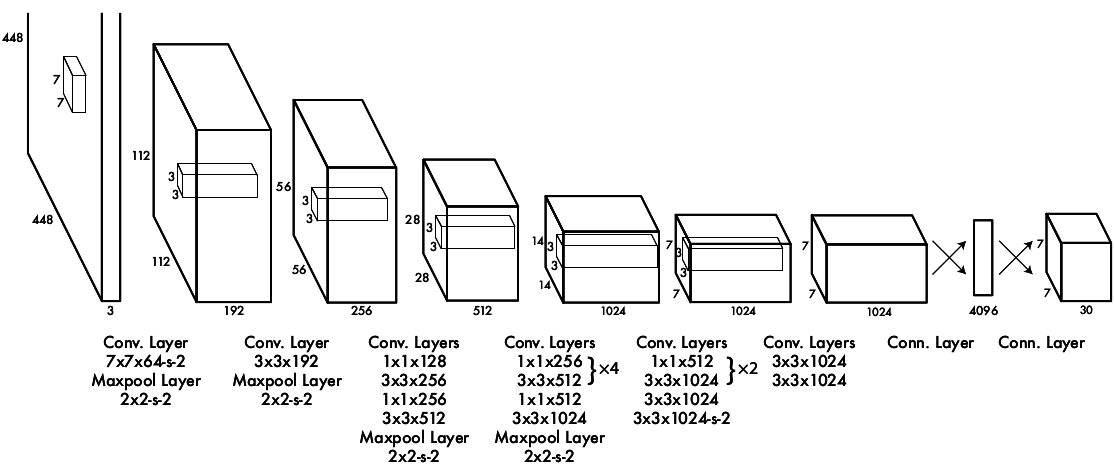
\includegraphics[width = \textwidth]{figures/YOLO/YOLO_architecture.png}
\caption[Αρχιτεκτονική YOLO]{Παράδειγμα της αρχιτεκτονικής YOLO \cite{6} για εικόνα εισόδου $224 \times 224$  όπου $S = 7, B = 2, C = 20 $. Το YOLO έχει 24 συνελεκτικά επίπεδα ακολουθούμενα από 2 ολικά συνδεδεμένα επίπεδα. Η χρήση $1 \times1 $ συνελεκτικών επιπέδων μπορεί να μειώσει τον χώρο των χαρακτηριστικών από τα προηγούμενα επίπεδα. Επίσης τα συνελεκτικά επίπεδα αρχικά εκπαιδεύονται στο ImageNet χρησιμοποιώντας τη μισή ανάλυση εικόνας ($224 \times 224$ εικόνα εισόδου) και μετά χρησιμοποιώντας τη διπλάσια για τον εντοπισμό αντικειμένων.}
\label{fig:YOLO_architecture}
\end{figure}

Ως συναρτήσεις ενεργοποίησης, αντί για τις πλέον διαδεδομένες \textit{ReLU} χρησιμοποιείται μια παραπλήσια μορφή: 

% \begin{equation}
$$
\phi(x) = \left\{ \begin{array}{cc}
    x, & x > 0 \\
    0.1 x, & \text{αλλιώς}
    \end{array}
    \right.
$$
% \end{equation}


Η εκπαίδευση γίνεται με κύριο σκοπό την βελτιστοποίηση του τετραγωνικού σφάλματος της εξόδου. Ως συνάρτηση απωλειών χρησιμοποιείται η συνάρτηση:

% \begin{figure}[H]
% \centering
% 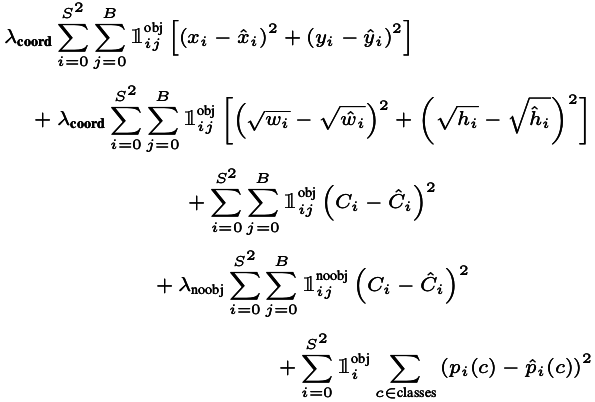
\includegraphics[width = 3in]{figures/YOLO/YOLO_lossFunction.png}
% \end{figure}
$$
\lambda_{coord} \sum_{i=0}^{S^2} \sum_{j=0}^{B} \mathbbm{1}_{ij}^{obj} \left[ (x_i-\hat{x_i})^2 + (y_i-\hat{y_i})^2\right]
$$
$$
   + \lambda_{coord} \sum_{i=0}^{S^2} \sum_{j=0}^{B} \mathbbm{1}_{ij}^{obj} \left[(\sqrt{w_i} - \sqrt{\hat{w_i}})^2 + (\sqrt{h_i} - \sqrt{\hat{h_i}})^2\right]
$$
$$
   + \sum_{i=0}^{S^2} \sum_{j=0}^{B} \mathbbm{1}_{ij}^{obj} (C_i - \hat{C}_i)^2
$$
$$
   + \lambda_{noobj} \sum_{i=0}^{S^2} \sum_{j=0}^{B} \mathbbm{1}_{ij}^{obj} (C_i - \hat{C}_i)^2
$$
$$
 + \sum_{i=0}^{S^2} \sum_{c \in \text{classes}} (p_{i}(c) - \hat{p}_{i}(C))^2
$$

Η εκπαίδευση γίνεται αρχικά με \textit{learning rate} $10^{-2}$ έπειτα $10^{-3}$ και τελικά $10^{-4}$. Επιπλέον χρησιμοποιείται η τεχνική \textit{dropout} \cite{3} με ποσοστό 50\%. Όλα αυτά οδηγούν σε ακρίβεια 63.4 mAP στο σύνολο δεδομένων PASCAL VOC 2007.
Η ταχύτητα αναγνώρισης αντικειμένων είναι 150 fps στη κάρτα γραφικών TITAN X της nvidia. Αντίστοιχα ο χρόνος που απαιτείται για την εκπαίδευση του νευρωνικού είναι μία εβδομάδα με το ίδιο hardware. 

Το YOLO στην πρώτη έκδοσή του πέτυχε παραπάνω από δύο φορές τη μέση ακρίβεια των συστημάτων αναγνώρισης αντικειμένων με καθυστέρηση $25 ms $. Αυτό του επιτρέπει να εισαχθεί και στο τέλος του δικτύου \textit{Fast R-CNN} για μια διορθωμένη αναγνώριση αντικειμένων στο φόντο της εικόνας. Στην παρουσίαση του δικτύου δεν γίνεται λόγος για απαίτηση μνήμης του συστήματος ωστόσο εκτελώντας τον αλγόριθμο από το \cite{8}, φαίνεται στο \cite{9} ότι όσο λιγότερη μνήμη υπάρχει διαθέσιμη τόσο πιο αργά εκτελείται ο αλγόριθμος. Από το Σχήμα \ref{fig:YOLO_architecture} υπολογίζεται πως για τον τανυστή εξόδου $ 7 \times 7 \times 30 $ απαιτείται μνήμη ίση με 808 MB για βάρη των 32-bit.
Αυτός μας δείχνει πως το YOLO είναι ένα βήμα προς την εισαγωγή των νευρωνικών στα ενσωματωμένα, ωστόσο πάλι απαιτεί αρκετή μνήμη και έχει περιορισμούς οι οποίοι δεν το χρήζουν κατάλληλο για κρίσιμες εφαρμογές. Παραδείγματα αδυναμιών του δικτύου είναι ότι τα περιβλήματα δεν υπολογίζονται πολλές φορές σωστά. Μια άλλη περίπτωση είναι ότι ενώ προσπαθεί να γενικευθεί για μικρά και μεγάλα αντικείμενα, όταν αυτά βρίσκονται σε εικόνες με διαφορετικές αναλογίες διαστάσεων ή επαναλαμβάνονται σε ένα γκρουπ με μικρές διαστάσεις αποτυγχάνει τον εντοπισμό τους.




\section{YOLO9000 \cite{7}}

Η βελτίωση αυτή του YOLO μπορεί να εντοπίσει αντικείμενα σε μια εικόνα από έως και 9000 διαφορετικές κατηγορίες. Μάλιστα, οι διαδικασίες μάθησης και εντοπισμού γίνονται πιο γρήγορα προσφέροντας και μεγαλύτερη ακρίβεια. Χαρακτηριστικό είναι ο λόγος 76.8 mAP στα 67 fps. Ωστόσο αντί να επεκτείνουν τις διαστάσεις του δικτύου, οι συγγραφείς προτίμησαν να το απλοποιήσουν δίνοντας τη δυνατότητα με διάφορες τεχνικές να διευκολύνουν την εκμάθησή του. Τα χαρακτηριστικά του δικτύου φαίνονται στον Πίνακα 1.1 και επεξηγούνται παρακάτω.

\begin{table}
\centering
% \captionof{table}{YOLOv2 features} \label{tab:title}
\begin{tabular}{c|c|c c c c c c c | c} 
& YOLO & \multicolumn{7}{c}{} & YOLOv2\\
\hline
batch norm & & \checkmark & \checkmark & \checkmark & \checkmark & \checkmark & \checkmark & \checkmark & \checkmark\\
hi-res classifier & & & \checkmark & \checkmark & \checkmark & \checkmark & \checkmark & \checkmark & \checkmark\\
convolutional & & & & \checkmark & \checkmark & \checkmark & \checkmark & \checkmark & \checkmark\\
anchor boxes & & & & \checkmark & \checkmark & & & & \\
new network & & & & & \checkmark & \checkmark & \checkmark & \checkmark & \checkmark\\
dimension priors & & & & & & \checkmark & \checkmark & \checkmark & \checkmark\\
location prediction & & & & & & \checkmark & \checkmark & \checkmark & \checkmark\\
passthrough & & & & & & & \checkmark & \checkmark & \checkmark\\
multi-scale & & & & & & & & \checkmark & \checkmark\\
hi-res detector & & & & & & & & & \checkmark\\
\hline
VOC2007 mAP & 63.4 & 65.8 & 69.5 & 69.2 & 69.6 & 74.4 & 75.4 & 76.8 & \textbf{78.6} \\
\end{tabular}
\caption[Χαρακτηριστικά του δικτύου YOLO9000]{Χαρακτηριστικά του δικτύου YOLO9000.}
\end{table}

\begin{itemize}
\setlength\itemsep{0em}

\item[] batch norm: Ο μέσος όρος αφαιρείται και διαιρείται με την τυπική απόκλιση όχι μόνο στην αρχή του δικτύου, αλλά και μέσα στο δίκτυο ανά κάποιες εισόδους.

\item[] hi-res classifier: Κατά την εκπαίδευση για κάποιες εποχές χρησιμοποιείται μεγαλύτερη ανάλυση της εικόνας $448\times448$ αντί $224\times224$.

\item[] convolutional (with anchor boxes): Χρησιμοποιούνται διαφορετικά περιβλήματα από ότι στην πρώτη έκδοση του νευρωνικού. Τα περιβλήματα αυτά είναι τα ίδια που περιγράφονται στο Faster R-CNN. Η διαφορά είναι ότι πλέον το δίκτυο εντοπίζει πάνω από 1000 κουτιά ανά εικόνα και αποκτά βελτιωμένο recall. Αυτή η δυνατότητα αντικαθιστά τα ολικά συνδεδεμένα επίπεδα στο τέλος του δικτύου.

\item[] dimension priors: Τα \textit{anchor boxes} έχουν το πρόβλημα πως οι αρχικές συνθήκες των βαρών εντοπισμού δημιουργούν μεγάλο πρόβλημα για την εκπαίδευση του συστήματος. Οπότε χρησιμοποιείται ο k-means για τον καθορισμό τους με k = 5 και μετρική:
$$ d(box,centroid) = 1 - IOU(box, centroid) $$

\item[] location prediction: Η εύρεση της θέσης του περιβλήματος παρουσιάζει αστάθεια. Για την αντιμετώπιση αυτού χρησιμοποιείται η μέθοδος άμεσου εντοπισμού θέσης με τη χρήση ενός ασαφούς ελεγκτή.

\item[] passthrough: Απλά ένα επίπεδο για την σύνδεση των δύο τελευταίων διότι κατά την εκπαίδευση αντικαθίσταται το τελευταίο επίπεδο συνέλιξης με $3 \times 3$ συνελεκτικά επίπεδα με 1024 φίλτρα το καθένα ακολουθούμενο από ένα τελευταίο $1 \times 1$ συνελεκτικό επίπεδο.

\item[] multi-scale: Το μέγεθος της εικόνας αυξάνεται ή ελαττώνεται κατά την εκπαίδευση.

\item[] hi-res detector: Ο εντοπισμός αντικειμένων γίνεται χρησιμοποιώντας καλύτερη ανάλυση της εικόνας από ότι το υπόλοιπο δίκτυο.

\end{itemize}


Η ταχύτητα του δικτύου οφείλεται στη χρήση τεχνικών του GoogleNet\cite{17}:
\begin{itemize}
  \setlength\itemsep{0em}
  \item Network In Network
  \item Global pooling
  \item $3\times3$ και $1\times1$ συνελεκτικά φίλτρα
\end{itemize}

Η δυνατότητα εντοπισμού πολλών κλάσεων οφείλεται στη χρήση ενός δέντρου που εμπεριέχει τις κλάσεις αυτές. Επομένως κάθε αντικείμενο έχει πολλές ετικέτες. Έτσι η τελική κλάση θα είναι κάποιο από τα φύλλα του δέντρου. π.χ. αν μια εικόνα δείχνει ένα "golden retreiver" τότε σίγουρα είναι αντικείμενο τύπου ζώου και τύπου σκύλου.
Με αυτό τον τρόπο δεν χρειάζεται να διαχωριστούν όλες οι κλάσεις μεταξύ όλων, αλλά αρκεί να εντοπιστεί ότι το αντικείμενο είναι τύπου 1 ή 2 και μετά να αναζητηθεί η σχέση μεταξύ των υπο-τύπων του έως ότου ο αλγόριθμος καταλήξει σε κάποιο φύλλο του δέντρου. Μάλιστα κατά την εκπαίδευσή του στο ImageNet για 1000 κατηγορίες αντικειμένων προστίθεται επιπλέον θόρυβος (διαφόρων ειδών) στις εικόνες ώστε να ενισχυθεί η ικανότητα εντοπισμού.
Τέλος, ενώ η πρώτη έκδοση του YOLO ήταν ένα πρώτο βήμα για την χρήση νευρωνικών σε ενσωματωμένα συστήματα, η δεύτερη αποτελεί ένα ικανοποιητικό και αρκετά αξιόπιστο σύστημα για την εφαρμογές όπως η αυτόνομη οδήγηση.

\section{R-CNN \cite{10}}

Το R-CNN ήταν από τα πρώτα δίκτυα που εμπνεύστηκαν από το AlexNet το έτος 2013. Οπότε και χρησιμοποιεί κομμάτια αυτού του δικτύου με μικρές αλλαγές. Ωστόσο προστίθεται παραπάνω λειτουργικότητα για την αναγνώριση πολλών αντικειμένων στην εικόνα και όχι πλέον μόνο για την κατηγοριοποίηση όλης της εικόνας ως ένα αντικείμενο. Για να το πετύχει αυτό το R-CNN χρησιμοποιεί τη τεχνική \textit{Selective Search} \cite{25}. Με αυτή μπορεί και εντοπίζει κάθε αντικείμενο στην εικόνα και το περιβάλει με ένα ορθογώνιο. Η εναλλακτική στρατηγική θα ήταν να χρησιμοποιείται ένα κυλιόμενο παράθυρο στην εικόνα για τον εντοπισμό των αντικειμένων. Η τελευταία αυτή τεχνική θα είχε μεγάλο υπολογιστικό κόστος έναντι της \textit{Selective Search}.

Μετά τον εντοπισμό των πιθανών περιοχών ύπαρξης αντικειμένων, οι περιοχές αυτές διαστασιοποιούνται σε τετράγωνες και χρησιμοποιείται μια επεξεργασμένη έκδοση του AlexNet για την κατηγοριοποίηση του αντικειμένου.

Στο τελευταίο επίπεδο του νευρωνικού υπάρχει ένα SVM το οποίο τελικά κατηγοριοποιεί το αντικείμενο σε κάποια κλάση (βήμα 4 στο Σχήμα \ref{fig:RCNN_overview}). Ωστόσο, όπως έχει αναφερθεί το R-CNN, αφού εκτελέσει το νευρωνικό, υλοποιεί και ένα ακόμη βήμα για βελτιστοποίηση των ορθογώνιων περιβλημάτων. Ουσιαστικά θεωρεί το πρόβλημα εύρεσης περιβλήματος ως πρόβλημα απλής παλινδρόμησης για να δώσει καλύτερα-στενότερα όρια στο περίβλημα. Έτσι στο τελευταίο βήμα λαμβάνει ως εισόδους τις περιοχές (τα ορθογώνια περιβλήματα) που υπάρχουν αντικείμενα και τις επιστρέφει βελτιωμένες.

Προφανώς το R-CNN δεν μπορεί να εκτελεστεί από κάποια ενσωματωμένη συσκευή, διότι χρησιμοποιεί το AlexNet. Ωστόσο, οι διάδοχοί του έχουν βελτιωθεί ώστε να είναι εφικτή η εκτέλεσή τους σε κάποια ενσωματωμένη συσκευή τόσο από άποψη μνήμης, όσο και από χρόνο εκτέλεσης.

\begin{figure}
\centering
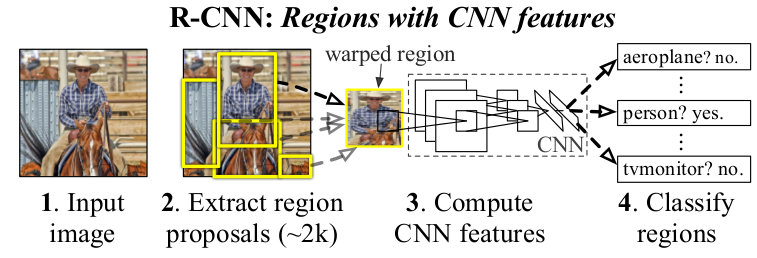
\includegraphics[width = \textwidth]{figures/RCNN/RCNN_overview.png}
\caption[Αρχιτεκτονική RCNN]{Πανόραμα του συστήματος εντοπισμού αντικειμένων του R-CNN \cite{10}. Το σύστημα λαμβάνει μια εικόνα (1), εξάγει 2000 προτεινόμενα περιβλήματα (2), υπολογίζει τα χαρακτηριστικά για κάθε ένα από τα περιβλήματα χρησιμοποιώντας ένα CNN (3), κατηγοριοποιεί κάθε περιοχή εντός κάποιου από τα προτεινόμενα περιβλήματα χρησιμοποιώντας linear SVM (4). Το R-CNN πετυχαίνει mAP ίσο με 53.7\% στο PASCAL VOC 2010 και 31.4 στο \textit{ILSVRC2013}.}
\label{fig:RCNN_overview}
\end{figure}

\section{Fast R-CNN \cite{11}}

Οι λόγοι για τους οποίους είναι αργό το R-CNN είναι δύο.
\begin{enumerate}
    \item Η χρήση του εμπρόσθιου περάσματος του AlexNet για κάθε πιθανού ορθογώνιου περιβλήματος από την Selective search το οποίο απαιτεί να εκτελεστεί το εμπρόσθιο πέρασμα του AlexNet περίπου 2000 φορές.
    \item Εκπαιδεύει τρία μοντέλα ξεχωριστά: το CNN για την εύρεση των χαρακτηριστικών της εικόνας, το SVM και το μοντέλο της απλής παλινδρόμισης για την βελτίωση των ορθογωνίων περιβλημάτων στο τέλος.
\end{enumerate}

Το Fast R-CNN υλοποιήθηκε με σκοπό να λύσει αυτά τα 2 προβλήματα και τελικά να επιταχύνει το R-CNN. Το πρώτο λύθηκε εκτελώντας τα βήματα σε διαφορετική σειρά. Πρώτα εκτελείται το εμπρόσθιο πέρασμα του CNN σε όλη την εικόνα και μετά γίνεται pooling σε κάθε πιθανό περίβλημα αντικειμένου (αυτό καλείται Region of Interest Pooling -RoIPool). Οπότε από περίπου 2000 εκτελέσεις του εμπρόσθιου περάσματος, πλέον απαιτείται μόνο μία. Το δεύτερο λύθηκε βάζοντας και τα τρία μοντέλα να εκτελούνται μαζί σε ένα κοινό δίκτυο. Η παλινδρόμηση γίνεται παράλληλα με την κατηγοριοποίηση η οποία πλέον δε γίνεται με SVM αλλά με \textit{Softmax classifier} λαμβάνοντας ως είσοδο το αποτέλεσμα του επίπεδου RoIPool. 

Η εκπαίδευση του δικτύου γίνεται 2.7 φορές πιο γρήγορα και οι χρόνοι αναγνώρισης αντικειμένων σε εικόνα ξεκινούν από 0.10 sec, ανάλογα με το μέγεθος της εικόνας. Η ακρίβεια (κριτήριο mAP) ελαφρώς αυξάνεται παρά τις αλλαγές στο δίκτυο.
Παρόλα αυτά οι χρόνοι εκτέλεσης συνεχίζουν να είναι απαγορευτικοί για ενσωματωμένα συστήματα. Επίσης δε γίνεται λόγος για κατανάλωση ενέργειας, διότι εκτελείται σε GPU (\textit{Nvidia K40 GPU overclocked to 875 MHz}). Επίσης αποφεύγεται η χρήση μεγάλων εικόνων, ώστε να μπορεί το δίκτυο να εμπεριέχεται ολόκληρο σε μια GPU και να μην απαιτείται πλέον χρήση του σκληρού δίσκου για caching. 

\begin{figure}
\centering
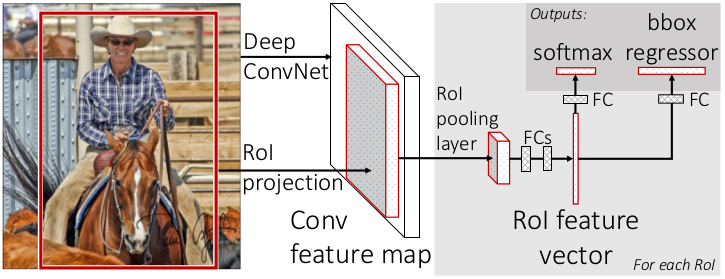
\includegraphics[width = \textwidth]{figures/RCNN/Fast-RCNN_architecture.png}
\caption[Αρχιτεκτονική Fast-RCNN]{Η αρχιτεκτονική Fast-RCNN \cite{11}. Η εικόνα εισόδου και οι πολλαπλές περιοχές ενδιαφέροντος (RoI) οι οποίες είναι είσοδοι σε ένα ενοποιημένο CNN. Κάθε RoI συλλέγεται σε ένα χάρτη χαρακτηριστικών δεδομένου μεγέθους και αντιστοιχίζεται σε ένα διάνυσμα χαρακτηριστικών χρησιμοποιώντας ολικά συνδεδεμένα επίπεδα (FCs στο Σχήμα \ref{fig:Fast_RCNN_architecture}). Το δίκτυο έχει δύο διανύσματα χαρακτηριστικών σε κάθε RoI. Ένα που προέρχεται από την έξοδο του Softmax και ένα από την γραμμική παλινδρόμηση. Τέλος το κομμάτι του ενοποιημένου δικτύου χρησιμοποιεί κοινή συνάρτηση απωλειών και όλα τα κομμάτια του εκπαιδεύονται μαζί.}
\label{fig:Fast_RCNN_architecture}
\end{figure}


\section{Faster R-CNN \cite{12}}
Η επόμενη -χρονικά- πρόταση ήταν το Faster R-CNN το οποίο προτάθηκε από το ερευνητικό τμήμα της \textit{Microsoft}. Το καινούριο αυτό δίκτυο βασίστηκε στο γεγονός ότι ο κύριος φόρτος εργασίας του Fast R-CNN γινόταν πλέον στον αλγόριθμο \textit{Selective Search}. Ταυτόχρονα, το βασικό δίκτυο επανα-υπολόγιζε χαρακτηριστικά (features) στις εικόνες στο πρώτο layer, τα οποία υπολόγιζε και η \textit{Selective Search} για να βρει τα περιβλήματα των αντικειμένων.

Επομένως η πρόταση για το Faster R-CNN ήταν η χρήση ενός νευρωνικού δικτύου RPN (\textit{Region Proposal Network}) το οποίο θα κάνει τη δουλειά της \textit{Selective Search}. Αυτό αποτελείται από δύο κομμάτια: ένα ολικά συνδεδεμένο επίπεδο που προτείνει περιοχές και τον ανιχνευτή του Fast R-CNN που χρησιμοποιεί τις προτεινόμενες περιοχές του πρώτου. Με αυτό τον τρόπο όλο το αρχικό R-CNN είναι πλέον ένα ενοποιημένο δίκτυο. Επιπλέον κατά τον εντοπισμό περιοχών αντικειμένων το RPN χρησιμοποιεί τη τεχνική της 'προσοχής'\cite{14} η οποία χρησιμοποιείται πλέον σε αρκετά νευρωνικά δίκτυα πέραν των συνελεκτικών για αύξηση της ακρίβειας.

\begin{figure}
\centering
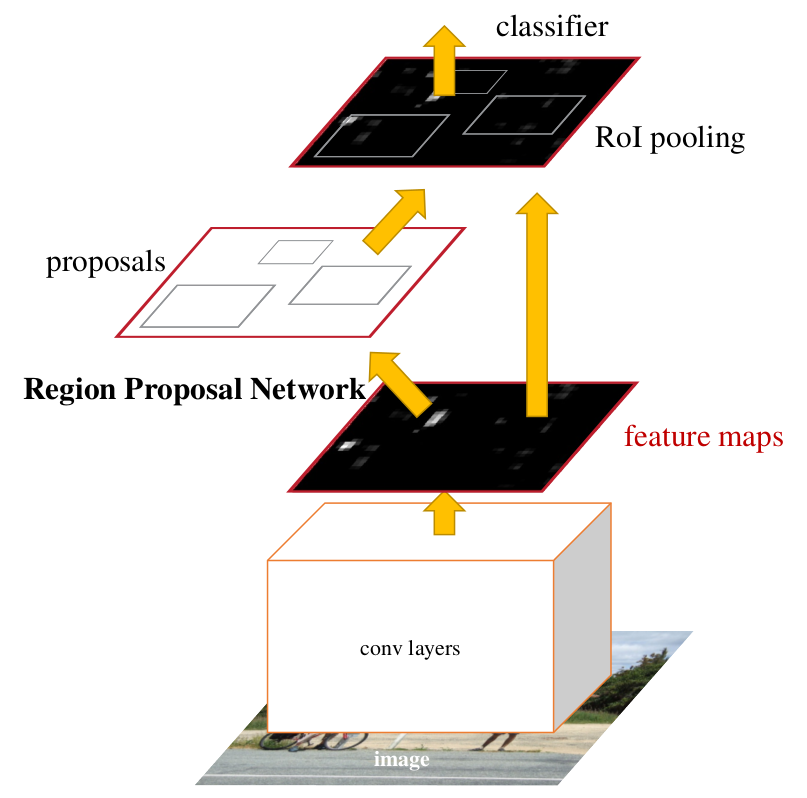
\includegraphics[width = \textwidth]{figures/RCNN/Faster-RCNN_RPN.png}
\caption[Η οντότητα RPN]{Η οντότητα RPN \cite{12}. Το δίκτυο Faster-RCNN είναι πλέον το ολοκληρωτικά ενοποιημένο δίκτυο για εντοπισμό αντικειμένων που εξελίχθηκε από το R-CNN. Η οντότητα RPN (\textit{Region Proposal Network}) βοηθά ως μέθοδος-τεχνική προσοχής αυτού του ενοποιημένου δικτύου, αντικαθιστώντας τη \textit{Selective Search}.}
\label{fig:Faster-RCNN_RPN}
\end{figure}

Αξιοσημείωτο είναι ότι το RPN χρησιμοποιείται από το SqueezeDet, αλλά αντί ολικά συνδεδεμένου δικτύου στο πρώτο χρησιμοποιεί συνελεκτικό επίπεδο. Και στις δύο περιπτώσεις υπάρχει ανεξαρτησία στη μετακίνηση των αντικειμένων.

Ουσιαστικά αυτό που συμβαίνει είναι ότι πάνω από τα αποτελέσματα του πρώτου επιπέδου τύπου CNN περνάει ένα παράθυρο το οποίο διαλέγει για κάθε εικονοστοιχείο της εικόνας $k$ πιθανά παράθυρα διαφορετικού μήκους και πλάτους. Οι χρόνοι εκτέλεσης είναι από 5 fps εώς 17 fps ανάλογα με τον τρόπο υλοποίησης του RPN σε GPU NVIDIA Tesla K40. Επίσης στο σύνολο δεδομένων \textit{PASCAL VOC 2012} πετυχαίνει ακρίβεια με κριτήριο mAP 59.9\%. H μνήμη ωστόσο συνεχίζει να αποτελεί πρόβλημα. Για αυτό δεν κρίνεται κατάλληλο για ενσωματωμένα συστήματα.

\section{Mask R-CNN \cite{13}}
Η τελευταία πρόταση βασισμένη στο R-CNN είναι το Mask R-CNN το οποίο προτάθηκε από την ερευνητική ομάδα της \textit{Facebook}. Το νευρωνικό δίκτυο αυτό είναι το Faster R-CNN με τη διαφορά πως αντί για ορθογώνια περιβλήματα των αντικειμένων πλέον εντοπίζει τα πραγματικά περιβλήματα στην εικόνα. Δηλαδή το σύνορο ενός αντικειμένου με την υπόλοιπη εικόνα δεν είναι πλέον ένα ορθογώνιο, αλλά ένα αφηρημένο σχήμα που το περιβάλλει με ακρίβεια εικονοστοιχείων. Για να επιτευχθεί αυτό χρησιμοποιείται ένας παράλληλος κλάδος του δικτύου, ο οποίος είναι υπεύθυνος για την κατηγοριοποίηση των εικονοστοιχείων σε αντικείμενα. Στο τέλος αυτού του κλάδου επιστρέφονται πίνακες οι οποίοι έχουν 1 στα εικονοστοιχεία στα οποία εντοπίζεται αντικείμενο και 0 σε αυτά που δεν εντοπίζεται. Κάθε πίνακας συνδέεται με ένα αντικείμενο σε ένα RoI. Αυτοί οι πίνακες είναι και οι μάσκες από όπου πήρε και το δίκτυο το ονομά του. Τέλος πρέπει να τονιστεί πως κάθε μάσκα βρίσκεται με παλινδρόμηση δύο κλάσεων αντικειμένων (δυαδική παλινδρόμηση) και όχι χρησιμοποιώντας \textit{Softmax}.

Προκειμένου να κατηγοριοποιηθεί ένα εικονοστοιχείο σε κάποιο αντικείμενο χρειάζεται να χρησιμοποιηθούν τα χαρακτηριστικά της εικόνας τα οποία υπολογίζονται χρησιμοποιώντας τα πρώτα συνελεκτικά επίπεδα του Faster R-CNN. Το πρόβλημα είναι πως οι διαστάσεις του τανυστή της εικόνας δεν είναι ίδιες με της διαστάσεις του τανυστή των χαρακτηριστικών. Έτσι αν μια περιοχή σημείων ήταν πάνω αριστερά και είχε διαστάσεις $15 \times 15$ πλέον θα έχει διαστάσεις $2.93 \times 2.93$ για χάρτη χαρακτηριστικών και εικόνα όπως παρουσιάζεται στο Σχήμα \ref{fig:Mask_RCNN_RoIAlign}. Σε αυτό το σημείο προτιμήθηκε να χρησιμοποιηθεί μια διγραμμική παρεμβολή, ώστε να υπολογίζονται τα χαρακτηριστικά των διαστάσεων με δεκαδικά. Αυτή η τεχνική λέγεται RoIAlign. Πρότερα, το εικονοστοιχείο που αντιστοιχούσε στη θέση $ x = 2.93$ των χαρακτηριστικών απλά θα αντιστοιχιζόταν στη θέση $ x = 2$.

\begin{figure}
\centering
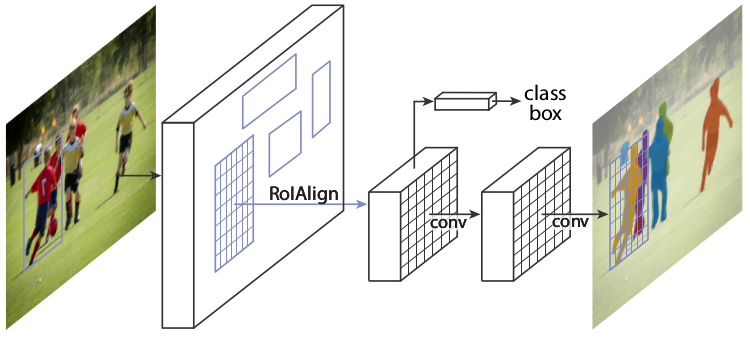
\includegraphics[width = \textwidth]{figures/RCNN/Mask-RCNN_RoIAlign.png}
\caption[RoIAlign]{Αντί του RoIPool, η εικόνα περνάει από το καινούριο επίπεδο RoIAlign \cite{13} ώστε οι περιοχές του χάρτη χαρακτηριστικών που διαλέγονται από το RoIPool να αντιστοιχούν με μεγαλύτερη ακρίβεια σε περιοχές της εικόνας εισόδου. Αυτό απαιτείται γιατί η κατηγοριοποίηση ανά εικονοστοιχείο  απαιτεί πιο λεπτομερή ευθυγράμμιση μεταξύ περιοχών της αρχικής εικόνας και του χάρτη χαρακτηριστικών.}
\label{fig:Mask_RCNN_RoIAlign}
\end{figure}

\begin{figure}
\centering
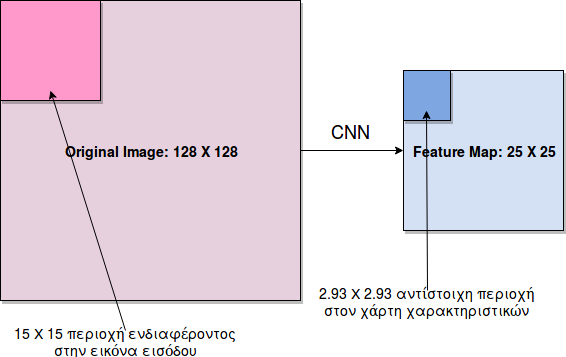
\includegraphics[width = \textwidth]{figures/RCNN/Mask-RCNN_RoIAlignExample.png}
\caption[Παράδειγμα RoIAlign]{Παράδειγμα αντιστοίχησης περιοχής από τον χάρτη χαρακτηριστικών στην αρχική εικόνα εισόδου. Για τον υπολογισμό των χαρακτηριστικών στο σημείο $(2.93, 2.93)$ χρησιμοποιείται διγραμμική παρεμβολή.}
\label{fig:Mask_RCNN_RoIAlignExample}
\end{figure}



Αυτή η κατηγοριοποίηση δίνει τη δυνατότητα για μεγαλύτερη ακρίβεια στον εντοπισμό αντικειμένων και φέρνει την αναγνώριση αντικειμένων πιο κοντά στα ανθρώπινα αποτελέσματα. Επιπλέον ο αλγόριθμος μπορεί να διαγωνιστεί και σε διαφορετικά περιβάλλοντα όπως το COCO όπου απαιτείται η κατηγοριοποίηση των εικονοστοιχείων από εικόνες σε αντικείμενα. Σε αυτό το σύνολο δεδομένων (COCO 2015, COCO 2016), η μέση ακρίβεια που επιτυγχάνει ο αλγόριθμος είναι $ mAP = AP = 37.1$, $ AP_{50} = 60.0 $, $AP_{75} = 39.4$, $ AP_S = 16.9$, $ AP_M = 39.9$, $ AP_L = 53.5 $ (μετρικές COCO \cite{15}). Η ταχύτητα εντοπισμού ανά εικόνα μένει ίδια στα 5 fps για το ίδιο hardware, διότι η καινούρια προσθήκη είναι ένα μικρό κομμάτι νευρωνικού δικτύου. Ταυτόχρονα, η μνήμη που χρειάζεται είναι περίπου η ίδια διότι το δίκτυο για τη μάσκα απαιτεί 355 kB το πολύ για Faster R-CNN τύπου FPN (Σχήμα \ref{fig:Mask_RCNN_architecture}).

\begin{figure}
\centerline{
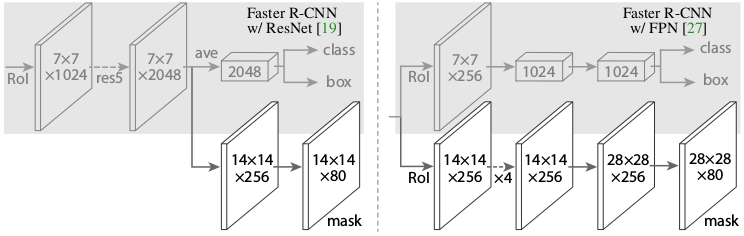
\includegraphics[width = \textwidth]{figures/RCNN/Mask-RCNN_architecture.png}
}
\caption[Αρχιτεκτονική Mask R-CNN]{Η αρχιτεκτονική Mask R-CNN \cite{13}. Η κεφαλή του δικτύου: Για την κεφαλή του δικτύου χρησιμοποιούνται κομμάτια από άλλα δίκτυα όπως το ResNet\cite{21} και το FPN\cite{22}. Τα βελάκια αντιστοιχούν σε συνέλιξη, αποσυνέλιξη ή πέρασμα από ένα ολικά συνδεδεμένο επίπεδο. Όλες οι συνελίξεις γίνονται από $3\times3$ φίλτρα, εκτός από τη συνέλιξη εξόδου, η οποία είναι $1\times1$. Οι αποσυνελίξεις γίνονται από $2\times2$ φίλτρα με βήμα 2. Επίσης η ενεργοποίηση χρησιμοποιεί ReLU στα κρυφά επίπεδα. Αριστερά φαίνεται η μάσκα του Mask-RCNN χρησιμοποιώντας το πέμπτο στάδιο του ResNet (res5) αλλαγμένο για περιοχή $7\times7$ με βήμα 1, αντί για $14\times14$ με βήμα 2. Δεξιά φαίνεται μια υλοποίηση της μάσκας του Mask-RCNN με τέσσερις διαδοχικές συνελίξεις πάνω στο Faster R-CNN με την κεφαλή του FPN.}
\label{fig:Mask_RCNN_architecture}
\end{figure}

Η εκπαίδευση γίνεται με τον ίδιο τρόπο όπως στο Fast R-CNN, χρησιμοποιώντας gradient descent με ορμή. Ωστόσο, τα RPN και το δίκτυο της μάσκας εκπαιδεύονται ξεχωριστά, θεωρώντας το RoI θετικό όταν η μετρική IoU είναι πάνω από 0.5. Επιπλέον τελικά χαρακτηριστικά που διερευνήθηκαν για το δίκτυο αυτό είναι:
\begin{itemize}
  \item Πολυκατηγορικές μάσκες ενάντια σε ανεξάρτητες μάσκες. Το αποτέλεσμα είναι ότι προτιμώνται οι ανεξάρτητες μάσκες οι οποίες μπορούν να υπολογιστούν μετά το RPN.
  \item Μάσκες ανά κατηγορία ή ανεξάρτητες. Το αποτέλεσμα είναι ότι οι ανεξάρτητες μάσκες έχουν πολύ μικρή διαφορά σε κριτήριο mAP από ότι αυτές που βρίσκονται ανά κατηγορία. Αυτό σημαίνει πως η πρόβλεψη μια μάσκας $ m \times m $ είναι πιο συμφέρουσα από ότι να έχω μία μάσκα για κάθε πιθανή κλάση του εντοπισμένου αντικειμένου.
\end{itemize}

Βέβαια λόγω των υπολογιστικών απαιτήσεων το δίκτυο αυτό δε θεωρείται κατάλληλο για ενσωματωμένα συστήματα. Παρ' όλα αυτά η δυνατότητα εντοπισμού αντικειμένων ανά εικονοστοιχείο το χρήζει πιο εύχρηστο για άλλους αλγορίθμους που χρησιμοποιούνται σε αυτά, όπως το SLAM με vision, η αυτόνομη οδήγηση κ.α. 



% \section{Inception-v4 \cite{17}}
% να δώσω έμφαση στο Inception module και στο πως μπορεί να γίνει retrain


% \section{ResNet}

\section{XNOR-Net \cite{18}}

Το δίκτυο XNOR προσεγγίζει διαφορετικά το πρόβλημα των CNN από ότι όλα τα παραπάνω. Η διαφορά έγκειται στη χρήση δυαδικών βαρών και αναπαράσταση της εισόδου ως δυαδικής. Η προσέγγιση αυτή καθιστά δυνατή την εκτέλεση του δικτύου όχι μόνο σε GPU ή εξειδικευμένο hardware όπως \textit{FPGA} ή \textit{ASIC}, αλλά και σε CPU. Περαιτέρω στην πρόταση του νευρωνικού εξετάζονται δύο εκδοχές
\begin{enumerate}
  \item Μόνο δυαδικά βάρη που δέχονται τιμές στο σύνολο $\{-1, +1\}$.
  \item Ταυτόχρονα δυαδικά βάρη και δυαδική είσοδος που δέχονται τιμές στο σύνολο $\{-1, +1\}$.
\end{enumerate}
Η δεύτερη από τις δύο εκδοχές είναι και η πιο αποτελεσματική, τόσο από άποψη χρόνου εκτέλεσης, όσο και από άποψη ακρίβειας. Και στις δύο περιπτώσεις η αρχιτεκτονική του δικτύου είναι ίδια με κάποιο άλλο π.χ. AlexNet\cite{20}, GoogleNet\cite{17}, ResNet\cite{21}. Αυτό που αλλάζει είναι τα βάρη και η σειρά με την οποία γίνονται οι πράξεις. Δηλαδή σε ένα κοινό δίκτυο έχουμε πρώτα τη συνέλιξη($C$), μετά την κανονικοποίηση($B$), αργότερα την ενεργοποίηση($A$) και τέλος τη συγκέντρωση ($P$). Στο δίκτυο XNOR η σειρά είναι διαφορετική: $B\rightarrow A\rightarrow C\rightarrow P$.

\begin{figure}
\centering
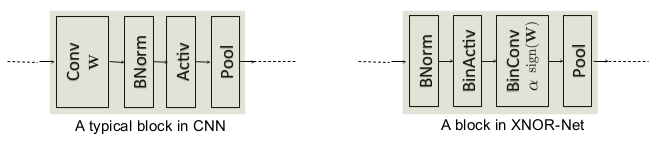
\includegraphics[width = \textwidth]{figures/XNOR_Net/XNOR_NET_block.png}
\caption[XNOR block vs typical CNN block]{Σύγκριση μεταξύ των μπλοκ του XNOR-Network (δεξιά) και ενός τυπικού CNN (αριστερά) \cite{18}.}
\label{fig:XNOR_NET_block}
\end{figure}

Για να είναι επιτυχής η προσαρμογή του δικτύου σε διάφορες αρχιτεκτονικές οι συγγραφείς επινόησαν έναν αλγόριθμο για το μετασχηματισμό της εισόδου και των βαρών στο σύνολο των δυαδικών τανυστών. Σε αυτό το σύνολο τανυστών τα στοιχεία κάθε τανυστή λαμβάνουν τιμές στο σύνολο $\{-1, +1\}$. Πιο αναλυτικά: Έστω η κανονική είσοδος ενός επιπέδου $I$ και έστω $W$ το σύνολο των βαρών αυτού του επιπέδου. Τότε σύμφωνα με τον προτεινόμενο αλγόριθμο:
    $$ \mathbf{I} \ast \mathbf{W} \approx (sign(\mathbf{I}) \circledast sign(\mathbf{W}) ) \odot \mathbf{K} \alpha  $$

Ο τελεστής $ \circledast$ αντιπροσωπεύει συνέλιξη με χρήση XNOR αντί για πολλαπλασιασμού.
Οπότε ο μετασχηματισμένος πίνακας εισόδου είναι ο $ sign(\mathbf{I}) $ και ο μετασχηματισμένος πίνακας βαρών είναι ο $ sign(\mathbf{W}) $.
Ο τελευταίος όρος είναι ένας πίνακας που πολλαπλασιάζεται στοιχείο ανά στοιχείο για να κλιμακωθεί σωστά το αποτέλεσμα της συνέλιξης ($  \circledast $) με XNOR.

\begin{figure}
\centering
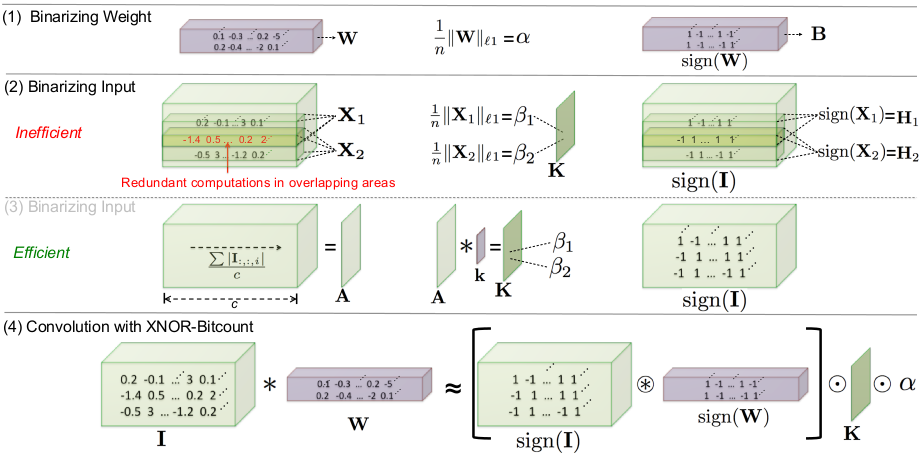
\includegraphics[width = \textwidth]{figures/XNOR_Net/XNOR_NET_procedure.png}
\caption[Αποτύπωση της συνέλιξης στο XNOR Net]{Επεξήγηση της διαδικασίας μετασχηματισμού της συνέλιξης σε συνέλιξη που κάνει χρήση της πράξης XNOR και δυαδικούς τανυστές \cite{18}.}
\label{fig:XNOR_NET_procedure}
\end{figure}

Όσον αφορά την εκπαίδευση το δίκτυο χρησιμοποιεί τη τεχνική ADAM \cite{19} και πετυχαίνει καλύτερη ακρίβεια από ότι αν χρησιμοποιούσε στοχαστική \textit{gradient descent} (\textit{SGD}). Επίσης είναι το πρώτο δυαδικό δίκτυο που έχει ελεγχθεί στο διαγωνισμό του \textit{ImageNet}. Στην ακρίβεια μεταξύ των κορυφαίων 5 κλάσεων χρησιμοποιώντας την αρχιτεκτονική του \textit{AlexNet} πετυχαίνει σκορ 69.2 και της κορυφαίας μίας 44.2. Αντίστοιχα χρησιμοποιώντας την αρχιτεκτονική του \textit{ResNet} πετυχαίνει 73.2 και 51.2. Αν χρησιμοποιούσε κανείς το \textit{ResNet} από μόνο του θα πετύχαινε ακρίβεια 89.2 για τις κορυφαίες 5 και 69.3 για τη κορυφαία μία. Βέβαια αυτή η θυσία της ακρίβειας γίνεται προς αύξηση της ταχύτητας, η οποία είναι ~$32\times$ φορές πιο αυξημένη. Μεγαλύτερη επιτάχυνση δικτύων επιτυγχάνεται όσο τα φίλτρα στα επίπεδα του νευρωνικού είναι μεγαλύτερα. Αυτό βέβαια βρίσκεται σε αντίθεση με τη πιο μοντέρνα τακτική να ελαττώνονται οι διαστάσεις των δικτύων όπως στο \cite{23}. 
Από πλευράς ενεργειακής αποδοτικότητας δε γίνεται λόγος στη σχετική έρευνα. Παρόλα αυτά, από τη στιγμή που το δίκτυο απαιτεί λιγότερες πράξεις από πολλαπλασιασμούς και είναι μικρότερο σε μέγεθος εξοικονομείται τόσο ενέργεια από τον επεξεργαστή όσο και από τη χρήση της DRAM.


\section{SSD \cite{26}}
Το δίκτυο αυτό παρουσιάζει κοινή αρχιτεκτονική με το Faster-RCNN και ουσιαστικά αποτελεί μια βελτίωση του (Deep Multibox \cite{27}). Η διαφορά του από άλλα δίκτυα είναι ότι διακριτοποιεί τις προβλέψεις για τα ορθογώνια περιβλήματα αντικειμένων σε ένα σύνολο από προκαθορισμένα aspect ratios και μεγέθη ανά περιοχή του (feature map). Κατά τον χρόνο εκτέλεσης το νευρωνικό εξάγει σκορ για την παρουσία κάθε κλάσης αντικειμένων σε κάθε ένα από τα προκαθορισμένα περιβλήματα και παράγει διορθώσεις ώστε κάθε περίβλημα να ταιριάξει στο μέγεθος του αντικειμένου. Επιπλέον το δίκτυο συνδυάζει προβλέψεις από πολλαπλά (feature maps) με διαφορετικές αναλύσεις για τη φυσική αντιμετώπιση αντικειμένων διαφόρων μεγεθών.

Το SSD είναι πιο απλό σε σχέση με τις μεθόδους που απαιτούν την ύπαρξη δικτύου για να προτείνει αντικείμενα, γιατί καταργεί εντελώς τα ξεχωριστά επίπεδα που παράγουν προτάσεις αντικειμένων και αυτά που τα ακολουθούν για αναδειγματοληψία ανά εικονοστοιχείο (ή ανά feature) και τοποθετεί όλους τους υπολογισμούς σε ένα δίκτυο. Αυτό καθιστά το δίκτυο εύκολο στην εκπαίδευση και στην ενσωμάτωση του σε άλλα συστήματα.

Οι πειραματισμοί στα σύνολα δεδομένων PASCAL VOC, COCO και ILSVRC επιβεβαιώνουν ότι το SSD έχει ανταγωνιστική ακρίβεια σε σχέση με άλλες μεθόδους που χρησιμοποιούν επιπλέον βήματα για την πρόταση του αντικειμένου. Ταυτόχρονα, είναι πιο γρήγορο και προσφέρει μια ενοποιημένη δομή τόσο για την εκπαίδευση όσο και για την απλή εκτέλεση. Για εικόνες εισόδου $ 300 \times 300 $ (SSD300) το δίκτυο επιτυγχάνει mAP 74.3\% στο σύνολο δεδομένων VOC2007 στα 59 FPS χρησιμοποιώντας την GPU Nvidia Titan X. Ενώ για εικόνες εισόδου $ 512 \times 512 $ επιτυγχάνει mAP 76.9\% υπερβαίνοντας την απόδοση του Faster-RCNN. 

Συγκρινόμενο με άλλες μεθόδους με ένα στάδιο, το SSD έχει κατά πολύ καλύτερη ακρίβεια ακόμα και με μικρότερη εικόνα εισόδου. Αυτό το χρήζει ικανό για να χρησιμοποιηθεί σε ενσωματωμένα συστήματα, αφού οι απαιτήσεις μνήμης του είναι μικρότερες, λόγω του μονού σταδίου και είναι αρκετά γρήγορο για την εκτέλεσή του. 

\section{Σύνοψη}
Στα προηγούμενα μέρη του κεφαλαίου αναλύσαμε κάθε δίκτυο ξεχωριστά παρουσιάζοντας την αρχιτεκτονική, την ακρίβειά και την ταχύτητά του. Επίσης, συμπεράναμε κατά πόσο το κάθε ένα μπορεί να χρησιμοποιηθεί σε ενσωματωμένη συσκευή. Από εκεί προέκυψε πως τα δίκτυα τα οποία μπορούν να χρησιμοποιηθούν για εντοπισμό αντικειμένων είναι τα:
\begin{itemize}
    \item SqueezeDet
    \item YOLO
    \item YOLO9000
    \item SSD
\end{itemize}

\subsection*{Από άποψη χρόνου εκτέλεσης}

Στη βιβλιογραφία διακρίνονται δύο είδη δικτύων: για εντοπισμό αντικειμένου (object localization) και για αναγνώριση αντικειμένου (object recognition). Τα πρώτα μελετούνται ως προς το χρόνο εκτέλεσης και την ακρίβεια (mAP). Τα δεύτερα ως προς τον αριθμό παραμέτρων, τον χρόνο εκτέλεσης, την ακρίβειά τους και το πόσο καλά μπορούν να εκπαιδευτούν. Επίσης, τα δίκτυα εντοπισμού εμπεριέχουν μέσα δίκτυα για εξαγωγή χαρακτηριστικών(feature extraction). Οπότε παρατίθενται οι δύο πίνακες για δίκτυα που κάνουν feature extraction (Πίνακας \ref{table:cnnComp}) και για δίκτυα που κάνουν εντοπισμό αντικειμένων (Πίνακας \ref{table:detCnnComp}).

Τα δίκτυα YOLO και SSD αν και προτείνονται για ενσωματωμένα, στα πειράματα που έχουν γίνει απαιτούν αρκετούς πόρους ακόμα και για ενσωματωμένες συσκευές, διότι εκτελούνται μόνο σε GPU. Επειδή γενικότερα στην βιβλιογραφία επικρατεί μία σύγχυση για τους χρόνους εκτέλεσης των νευρωνικών δικτύων στο παρόν κείμενο χρησιμοποιήθηκε η μετρική frame/ms/Watt , όπου μετριέται ο χρόνος εκτέλεσης ως προς την κατανάλωση ισχύος στο 'forward pass' του νευρωνικού ανά frame. Κατά αυτό τον τρόπο υπάρχει ένα μέτρο το οποίο μπορεί να συγκρίνει τους χρόνους εκτέλεσης ανεξαρτήτως της αρχιτεκτονικής. Ωστόσο, υπάρχει το μειονέκτημα ότι διαφορετικές αρχιτεκτονικές χρησιμοποιούν διαφορετικά ποσά ενέργειας για να πραγματοποιήσουν τις ίδιες πράξεις.


Από άποψη ακρίβειας το επικρατέστερο δίκτυο (από αυτά που αναλύονται) είναι το Faster-RCNN. Παρόλα αυτά, τα δίκτυα δεν μπορούν να συγκριθούν με το Mask-RCNN γιατί αυτό δεν βρίσκει ορθογώνια περιβλήματα μόνο αλλά κάνει και εντοπισμό των αντικειμένων της εικόνας ανά εικονοστοιχείο. Για τα υπόλοιπα η σειρά ακρίβειας είναι η παρακάτω.
\begin{enumerate}
    \item Faster-RCNN
    \item SqueezeDet
    \item YOLO9000
    \item SSD
    % \item XNOR-Net
\end{enumerate}

Αξιοσημείωτο είναι ότι το SSD πετυχαίνει καλύτερη ακρίβεια, όση και το Faster-RCNN με χρόνους εκπαίδευσης διπλάσιους του YOLO. Επίσης ότι το SqueezeDet μπορεί και ξεπερνάει την ακρίβεια του Faster-RCNN σε κάποια σύνολα δεδομένων. Το τελευταίο στη λίστα είναι το δίκτυο XNOR-Net το οποίο έχει μεγάλη διαφορά από τα άλλα δίκτυα σε ακρίβεια. Όπως αναφέρεται και στη σχετική δημοσίευση \cite{18}, το XNOR-Net προσπαθεί να λύσει το πρόβλημα εκτέλεσης νευρωνικού σε CPU χρησιμοποιώντας bits για την αναπαράσταση των παραμέτρων του και όχι Bytes, προκειμένου να το χωρέσει στη διαθέσιμη μνήμη που διαθέτει μία συμβατική ενσωματωμένη συσκευή. Η χρησιμότητα του όμως αίρεται στη γενική περίπτωση, με τη λογική ότι το SqueezeDet μπορεί να πετύχει αρκετά μεγαλύτερη ακρίβεια έχοντας μικρότερο μέγεθος. Χρήσεις του XNOR-Net αφορούν περισσότερο σχεδιαστικά προγράμματα π.χ. για αναγνώριση αντικειμένων από σκίτσα \cite{33}.

\subsection*{Από άποψη μνήμης}
Τα δίκτυα για feature extraction μελετώνται πλέον με τον αριθμό των παραμέτρων. Αυτό γίνεται διότι η αναπαράστασή τους σε 8, 16 ή 32 bit καθορίζεται από τους επιπλέον αλγόριθμους συμπίεσης (π.χ. Ristretto \cite{28}). Ο Πίνακας \ref{table:cnnComp} δείχνει τα χαρακτηριστικά κάθε νευρωνικού τέτοιου τύπου. Οι χρόνοι αφορούν την εκτέλεση των δικτύων αυτών με τη χρήση του tensorflow \cite{34} στη GPU GTX 1080 Ti της NVIDIA, και στο σύνολο δεδομένων του Imagenet ILSVRC2012. Οι υπολογισμοί τους έγιναν για το σκοπό αυτής της διπλωματικής στη συστοιχία του εργαστηρίου Αρχιτεκτονικής και συστημάτων που αναλύεται σε παρακάτω κεφάλαιο. Παρά ταύτα, παρατίθενται και οι χρόνοι για δίκτυα που δεν ενδείκνυται η εκτέλεσή τους σε GPU, σε άλλη πλατφόρμα.


\begin{table}
\centering
% \captionof{table}{YOLOv2 features} \label{tab:title}
\begin{tabular}{c|c|c|c} 
 Δίκτυο feature extraction & Top-1 ακρίβεια & Αριθμός Παραμέτρων & frames/ s /W \\
\hline
% SqueezeNet & 57.5 & 421,098 (6 bit) & $68.4\, ms / 2W$ \\ % NAO ATOM
SqueezeNet & 57.5 & 421,098 (6 bit) & $ 9.429 $ \\ % GTX 1080 Ti
XNOR-Net & 44.2 & 61M (61MB) & $439.56 \text{fps}\, / 2W$ (ATOM Z530 CPU) \\ % 
VGG-16 & 70.5 & 14,714,688 & $2.225$ \\ %GTX 1080 Ti
MobileNet-224 & 83.3 & 3,191,072 & $45.278$ \\ %
ResNet-101 V2& 76.4 & 42,605,504 & $2.316$ \\ %GTX 1080 Ti
% Inception V2 & 73.9 & 10,173,112 & \\
Inception V3 & 78.0 & 21,802,784 & $ 2.4276$ \\  %GTX 1080 Ti
Inception V4 & 80.4 & 54,336,736 & $ 1.3816$ \\ %GTX 1080 Ti, Inception V4
\hline
\end{tabular}
\caption[Σύγκριση δικτύων για feature extraction]{Σύγκριση δικτύων για feature extraction στο εμπρόσθιο πέρασμα για ένα frame. Όλα τα δίκτυα έχουν παραμέτρους σε αναπαράσταση float32 εκτός από το XNOR-Net και μόνο αυτό εκτελείται σε CPU. Η ακρίβεια των δικτύων μετριέται στο σύνολο δεδομένων του ImageNet. Τα χαρακτηριστικά των δικτύων που δεν αναλύονται στο κεφάλαιο είναι από \cite{28}, ενώ άλλα προέρχονται από \cite{29}, 
\cite{30, 31, 32}. Οι εικόνες για την μέτρηση είναι στο μέγεθος των εικόνων του ImageNet. Αν η πλατφόρμα εκτέλεσης του δικτύου είναι διαφορετική, τότε αυτή αναγράφεται μέσα σε παρενθέσεις. Οι παραπάνω υπολογισμοί έγιναν στη συστοιχία του εργαστηρίου, εκτός από αυτούς που δίνονται για το XNOR-Net οι οποίοι υπολογισμοί έγιναν σε επεξεργαστή \textit{ATOM Z530}.}
\label{table:cnnComp}
\end{table}

\begin{table}
\vspace{-5em}
% \centering
\begin{tabular}{c|c|c} 
 Δίκτυο Εντοπισμού & mAP & Χρόνος Εκτέλεσης / frame / W \\
\hline
SqueezeDet + SqueezeNet & 80.4 (KITTI)&$31.2\, ms / 128.3 W$ (NVIDIA Titan X)\\ % 
YOLO9000 $480\times480$ + Darknet & 77.8 (PASCAL VOC 7+12) & $ 17\, ms / 250 W$ (NVIDIA Titan X) \\ % 
% XNOR-Net & 44.2 () & $2.275 ms\, / 2W$ (NAO ATOM) \\ % 
SSD300 + VGG16 & 74.3 (PASCAL VOC 7+12) & $ 52\,ms / 250 W$ (NVIDIA Titan X) \\
Mask R-CNN + ResNeXt-101 & 37.1 (MS COCO 2015) & \~$240\,ms / 143.1 W$ (NVIDIA Titan X)\\
Faster R-CNN + ResNet & 76.4 (PASCAL VOC 7+12)& $200\,ms / 143.1 W$ (NVIDIA Titan X)\\
\hline
\end{tabular}
\caption[Σύγκριση δικτύων για εντοπισμό αντικειμένων]{Σύγκριση δικτύων για εντοπισμό αντικειμένων. Η ακρίβεια των δικτύων μετριέται σε διάφορα σύνολα δεδομένων. Η παράθεση αυτή γίνεται, διότι δεν υπάρχει κάποιο κοινό σύνολο δεδομένων στο οποίο να έχουν εκτελεσθεί όλα τα δίκτυα εντοπισμού, σε αντίθεση με τα απλά CNN. Βέβαια αυτό γίνεται για λόγους που αφορούν την ακρίβεια και θα εξετασθούν αναλυτικότερα στο επόμενο κεφάλαιο.}
\label{table:detCnnComp}
\end{table}

Το RCNN και οι απόγονοί του τοποθετήθηκαν κυρίως για να φανεί η σειρά στην οποία όλοι βασίστηκαν κατά την ανάπτυξη των νευρωνικών δικτύων εντοπισμού αντικειμένων. Όλες οι παραπάνω προτάσεις συγκρίνονται με τα Fast-RCNN και Faster-RCNN και όπως φαίνεται τα επόμενα θα συγκριθούν με το Mask-RCNN. Μάλιστα όπως το SqueezeDet εμπνεύστηκε από το Faster R-CNN έτσι και ένα επόμενο δίκτυο ενσωματωμένων μπορεί να εμπνευστεί από το Mask R-CNN. Ήδη παρόμοια λειτουργία σε ενσωματωμένα συστήματα πραγματοποιεί το ENet \cite{16}.
